%----------------------------------------------------------------------------------------
%	PACKAGES AND OTHER DOCUMENT CONFIGURATIONS
%----------------------------------------------------------------------------------------

\documentclass[12pt]{article}
\usepackage{graphicx}
\usepackage[utf8]{inputenc}  
\usepackage[T1]{fontenc} 
\usepackage[top=1.5cm,bottom=1.5cm,left=1.3cm,right=1cm,asymmetric]{geometry}

\usepackage{amsfonts}
\usepackage{graphicx}
\usepackage{amsmath}
\usepackage{fancyhdr}
\usepackage{array,multirow,makecell}
\usepackage{cancel}
\usepackage{subfig}
\usepackage{wrapfig}
\setcellgapes{1pt}
\makegapedcells
\newcolumntype{R}[1]{>{\raggedleft\arraybackslash }b{#1}}
\newcolumntype{L}[1]{>{\raggedright\arraybackslash }b{#1}}
\newcolumntype{C}[1]{>{\centering\arraybackslash }b{#1}}

\pagestyle{fancy}
\renewcommand{\footrulewidth}{1pt}
\fancyhead[R]{\textit{Master MVA : Probabilistic graphical models}}
\fancyfoot[L]{\textit{}}
%\usepackage{unicode-math}
%\setmathfont{XITS Math}
%\setmathfont[version=setB,StylisticSet=1]{XITS Math}


%\geometry{hmargin=1.5cm,vmargin=2cm}   

\begin{document}
\section*{Latent dirichlet allocation for label modelling}
\section*{Thibaud Ehret \& Sammy Khalife}
~\\
\section*{Presentation of the model [Journal of Machine Learning, 2003]}
\begin{figure}[!h]
\centering
\captionsetup{justification=centering,margin=2cm}
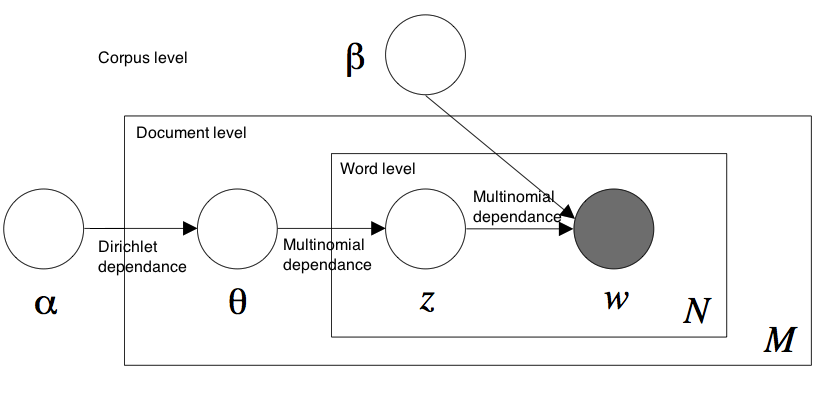
\includegraphics[width=13cm]{LDA.png}
\caption{Graphical model associated to Latent dirichlet association}
\end{figure}
~\\
In the latent dirichlet model (LDA), there are different levels of representation of the object concerned (documents in our case). It differs from a simple multinomial model in the sense that each object can be associated with multiple topics. ~\\
~\\
\textbf{Generation of documents}~\\
~\\
The parameter $\theta$  which belongs to $\mathbb{R}^{d}$ is sampled once per document from a smooth distribution on the topic simplex, and represents the distribution of the topics within the document. $\theta$ is generated through a dirichlet distribution of parameter $\alpha$. We suppose that each word $\textbf{w}$ is generated through a multinomial probability conditionned on the topic : $\beta \in \mathbb{R}^{K*V}$, with $\beta_{ij}=p(w^{j}=1|z^{i}=1)$, V representing the number of possible words, and K the number of topics.
\begin{eqnarray*}
p(\textbf{w}|\alpha, \beta) &  = & \int p(\theta | \alpha, \beta)p(\textbf{w} | \alpha, \beta, \theta)d\theta\\
\end{eqnarray*}
In the LDA model, we have $ \theta \perp \beta$, and $p(w_{i} | \alpha, \beta, \theta) \perp p(w_{j} | \alpha, \beta, \theta)$  for $ i \neq j $
\begin{eqnarray*}
p(\textbf{w}|\alpha, \beta) & = & \int p(\theta | \alpha) \prod_{n=1}^{N} p(\textbf{w}_{n} | \alpha, \beta, \theta)d\theta\\
& = & \int  p(\theta |\alpha) \prod_{n=1}^{N}  \sum_{z_{n}}p(z_{n}|\alpha, \beta, \theta)p(\textbf{w}_{n} | \alpha, \beta, \theta, z_{n}) d\theta\\
\end{eqnarray*}
Moreover $z \perp (\alpha,\beta)$ and $\textbf{w}_{n} \perp (\alpha,\theta)$, then
\begin{eqnarray*}
p(\textbf{w}|\alpha, \beta) & = & \int p(\theta | \alpha)  \prod_{n=1}^{N}  \sum_{z_{n}}p(z_{n} |\theta)p(\textbf{w}_{n} | z_{n}, \beta) d\theta\\
\end{eqnarray*}

\section*{Inference and parameter estimation}
Then the natural inferential problem that we need to solve in order to use LDA, is to compute :
$$p(\theta, \textbf{z}|\textbf{w},\alpha,\beta)=\frac{p(\theta,\textbf{z},\textbf{w}|\alpha,\beta)}{p(\textbf{w}|\alpha,\beta)}$$
Unfortunately, this expression is intractable due to the coupling between $\theta$ and $\beta$.
Then, the following EM scheme is used to make an inference on parameters $\alpha$ and $\beta$ : ~\\
~\\
-Get the tightest lower bound of the actual log-likelyhood among the simplified model :~\\
\begin{figure}[!h]
\centering
\captionsetup{justification=centering,margin=2cm}
\includegraphics[width=7cm]{EM}
\caption{Approximation model for best lower bound approximation}
\end{figure}
~\\
-Parameter estimation of $\alpha$ and $\beta$ by maximizing the lower bound with respect to $\alpha$ and $\beta$~\\



\end{document}